

\section*{A Preface on Humanity and the Climate}
\begin{flushleft}\emph{
The development of humanity is not unlike the chirography of an Aristotelian tragedy. It starts with a simple/primitive species cradling a noble cause - to improve their chances of survival. Here the protagonist (humankind) develops a fatal flaw: an insecurity and latent distruction of their home due to a sudden rise to power. 
Having acknowleged this flaw, we now strive to imporve our understanding of the universe, correct past mistakes and stem the tide of inevitable change. \vspace{\baselineskip}\linebreak
With tragedy being an imitation not of humanity, but of action and life, happiness and misery, it is only expected that such a comparison to our current affairs should stir feelings of catharsis when exploring our need for research and scientific advancement. 
It is with that I begin this thesis with the begining of the planet, its atmosphere and consequently the beginning of humankind. 
}
\end{flushleft}

\section{Whence} 
This section describes the intial formation of an atmosphere, how this led to life, and ultimately the human race. 
\subsection{Formation of the Atmosphere}
 4.5 billion years ago the earth was part of a disk of dust and gas orbiting our sun. As these gasses move about, resonant drag instability led to the clumping of dust particles, \cite{drag,planet}. As these `clumps' become denser, other forces come in to play, further increasing the size - eventually forming the hot mix of gas and solid which became the Earth. 

As it cooled, this Earth becan to accumelate an atmosphere of primodial gasses from the vollotile componenets of the gas cloud. These gasess were then supplemented through outgassing (volcanic eruptions). At this point in time oxygen was not only absent in the atmopshere, but also had many siks within the Earths anoxidised crust. It was not until oxygenic photosynthesis (\cite{oxygenicphotosynthesis}) that the concentrations of oxygen in the atmosphere started to increase. Eventually the development of multicellular cyanobacteria\footnote{The phylum of phtosynthetic prokaryotic (cells not containing a distinct nucleus) bacteria - e.g. blue-green algae} resulted in biologically induced oxygen accumelating in the atmosphere, \cite{multicellular}. This led to the most significant climate event in the planets history: the Great Oxigenation Event (2.5 billion years ago), \cite{oxidation}. This increase of oxygen allowed oragnisms to become larger and more active, eventually resulting in the human race. 

\subsection{Rise of the Homo Spiens (`Wise Man')}
About x million years ago there were many varieties of the homo genus. With the development of the human brain, energy transfer changed. A larger brain required more fuel, and therefore with the development of cooking\footnote{The first known case of indoor air pollution} humans were able to increase their... 

This led to the first know source of indoor air pollution. 


With the this increased capability, a language capable of communicating information, allowing for the ability to not only hunt larger prey but also. 
Ability to metaphorical, allowed fruther knwoplege transfer , cvave paings and metaphoirical for people over 150 .... 

REFERENCES TO OTHER CHAPTERS... 
- vis 
- accounting via metaphors
- and an interest in science, and atmosphere 

\section{Motivation}

Air pollution and climate have always been a concern for the human race. Concerns about lead in the air can be documented back as far as 6000 years ago [se ref, ], in ancient Rome [1145] and in 1285 where after a visit from Queen of England to a coal burning to Nottingham, the first air pollution act was deployed [1147]. Modern day




air pollution = animals

air qulaity pollicy
kingxx

\begin{figure}[H]
  \centering
  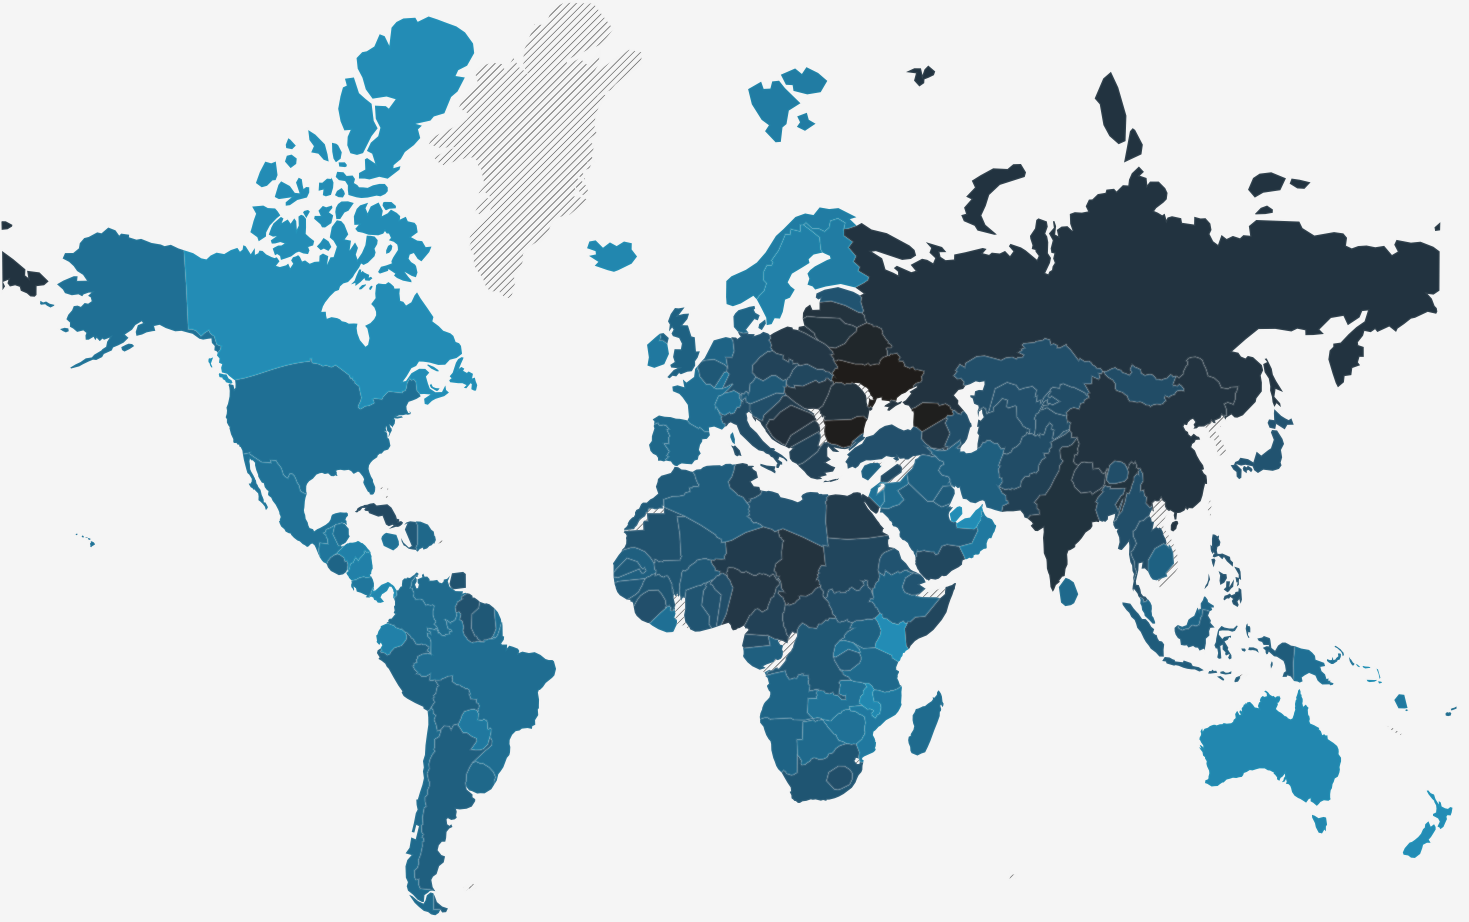
\includegraphics[width=\textwidth]{who.png}
  \caption{\textbf{Deaths attributed to air pollution REF WHO 16}}
  \label{fig:who}
\end{figure}




\section{Ozone and its role}
Ozone has two roles within the atmosphere. High up in the stratosphere it servers as a barrier to dangerous ultraviolet radiation. The importance of this was discovered in (HOLE PAPER) where the release of CloroFlouroCarbons from deodorants produced ...

However within the troposhere (<15k?) the production and loss of ozone has a direct impact on human life. Polluted environments, such as industrial London,
SMOG, Clean air act. 



\section{The NOx cycle}
Nitrogen Oxides (NOx) come predominantly from motor verhicles and power stations and can cause respiotory problems in children and asmatics [se1261]. They also play an important role in the formation and destruction of ozone.



\section{Changing Climate}



The main removal

\subsection{HOx Cycle}








VOC


\section{Modelling the Earth}
In the previous section the air quality and its detrimental effects on human health was seen to influence polcicy for cities and industry. Koyoto, Islands suing powerstations.

For a policy to be passed there needs to not only evidence of the problem, but a strong suggestion that any proposed changes will have the desired effect. As it is not possible to perform experiments on complex, and often unknown, chemistry at every location on the planet, we are forced to rely on the numerical simulation of the Earth System, and the constituent parts within it.

\subsection{Earth System Models (ESM)}

  ESMs are models capable of predict past or future interactions of the planetary system. They represnt our foremost understanding of the complex interplay between land-surface (geosphere), ocean (hydrosphere), ice (cryosphere) and the air (atmosphere), and act as a surrogate to manual experimentation -  which is just not possible on the global scale.

ESMs can also be split into their individial parts. One example of this is the Chemistry section of the Goddard Earth Observing System (an integrated ESM and data assimulation model hosted by NASAs Goddard space flight centre [CITE]) - GEOS Chem. GEOS-Chem is a global 3D model of atmospheric chemistry which is driven by the meteorology provided by NASA [CITE]. Here the earth is split up into cubic sphere cells longitudally and latitudally, as well as vertically FIG CELLS\footnote{This image is not from GEOS-Chem.}. Each one of these cells performs several purtubations of the chemistry within them, before any long-lived species are transported, and the process is repeated. If extracted separately a single one of these cells may be used to explore the sensetivity of different species for a range of input conditions. This is the bases of the atmospheric box model.


\subsection{The zero-degree box model.}
A box model



mechanism,

integrator,

etc.






\subsubsection{Chemical Mechanisms}
The atmosphere consists of thousands of species, with tens of thousands of reactions between them.

These models represent real wodlc reactions


In modelling these we can describe their rate of production and loss with respect to the species they react with.



\subsection{The model development cycle}
Scientific understanding is the product of many cycles of trial and error, \autoref{fig:devcycle}. In atmospheric chemistry we start with a hypothesis or a question, e.g. will changing X have a negative response on Y. We then construct a theoretical model to represent the chemsistry within. This chemistry is updated to reflect the rates and reactions that have been recorded in laboratory/chamber experiments. This cycle is then repeated until the model and real-world observations produce a comparable result.

\begin{figure}[H]
    \centering
    
\includegraphics[width=0.6\textwidth]{devcycle.png}
    \caption{\textbf{The scientific development cycle.}This shows the iterative nature between modelling, observation and laboratory experimentation}
    \label{fig:devcycle}
\end{figure}






ESM

 A series of box models.


 \subsection{The Dynamically Simple Model of Atmospheric Chemical Complexity}








 % Early simulations, such
 %
 % as those run on ENIAC2, were capable of success-
 % ful 24 hour weather prediction. Unfortunately, al-
 % though a great feat, the delay in simulation time re-
 % sulted in a computation that only just kept up with
 %
 % real-life events [Lynch, 2008]. in 1995 a general circu-
 % lation model of the atmosphere was created by Phillips
 %
 % [Phillips, 1956]. It was soon discovered that this was
 % insu
 % cient to represent the Earth, and a general Global
 % Climate Model (GCM) was formed from the union
 % of atmospheric, oceanic, cryospheric and land-surface
 %
 % models [NIPCC, 2010]. The outcome of this was a pro-
 % gram capable of simulating accurate short-term weather
 %
 % predictions, which can allow an insight into the con-
 % tributing factors of climate change.
 %
 %
 % \subsubsection{Common Problems with Earth prediction}
 % There are several problems that an earth simulation model can face, most of which can be attributed to computational efficiency. An example of this is seen with the
 %
 % MET - DAY TO SIMULATE
 %
 % Other problems with meteorlogy that are encountered rest on resolution. Too fine a scale and the model can take forever to run. simplfy, lose local effect and islands.
 %
 % Finally the tuning of models can result in overfitting due to a limited understanding or dataset. Here a model may be tweked to ..
 %
 % Numerical stiff chemical complexity.
 %
 %

\section{Thesis Layout}
This thesis will explore a series of methods for describing and understaning the complex chemistry which may exist as part of an atmospheric chemistry mechanism. The mechanism used is a near-explicit representation of our foremost understanding of how gas phase chemistry in the troposphere reacts - the Master Chemical Mechanism, \citep{mcm}.

We begin by exploring the use of visualisation to convey complex scientific data (\autoref{ch:vis}). Next we apply this to the representation of species in a mechanism, and the relationships between them. To do this it is found that the node-link style graph format is the most beneficial, the use of which is then explored further (\autoref{ch:graph}). \autoref{ch:}
